\documentclass{article}
\usepackage[preprint,nonatbib]{neurips_2024}
\usepackage{pgfplots}
\usepackage{graphicx}
\usepackage{algpseudocode}
\usepackage{algorithm}
\usepackage{amsmath}





\title{Contextual Morphogenesis in Large Language Models: A Novel Approach to Self-Organizing Token Representations}





\author{
Alistair Dombrowski \And
Beatrix Engelhardt \And
Dimitri Fairbrother \And
	Henry Evidail 
}


\begin{document}



\maketitle


\begin{abstract}
Token representations influence the efficiency and adaptability of language models, yet conventional tokenization strategies impose rigid segmentation boundaries that do not adjust dynamically to evolving contextual relationships. The introduction of contextual morphogenesis establishes a self-organizing mechanism that restructures token boundaries based on learned contextual dependencies, allowing embeddings to evolve progressively across iterative processing steps. Empirical evaluations demonstrate that dynamically adjusted tokenization contributes to reductions in perplexity while maintaining representational stability, particularly in linguistically complex domains where static segmentation fails to capture nuanced dependencies. Computational trade-offs associated with self-organizing token structures indicate that additional processing overhead remains within feasible limits, provided that optimization strategies account for segmentation update efficiency. Comparative assessments across different linguistic corpora suggest that adaptive tokenization preserves interpretability while improving alignment with contextual cues, reinforcing the potential of morphogenetic segmentation mechanisms to refine predictive accuracy. Stability analyses confirm that evolving token structures maintain consistent segmentation behaviors across varied text distributions, ensuring that representational adaptations remain linguistically coherent. The effectiveness of contextual morphogenesis in refining structural stability and predictive performance highlights its viability as an alternative to traditional tokenization methods. Further analysis of computational efficiency considerations suggests that hybrid strategies integrating both static and dynamic segmentation techniques may offer a balanced approach to optimizing representational flexibility while maintaining inference efficiency.


\end{abstract}




\section{Introduction}

Language models have undergone significant advancements, progressively shifting from rudimentary probabilistic frameworks to sophisticated neural architectures capable of processing vast amounts of text. The evolution of these models has been largely driven through innovations in deep learning, particularly through transformer-based architectures that allow for more efficient handling of long-range dependencies in text. As research continues to refine the efficiency and scale of such models, one of the fundamental challenges that persists involves the manner in which token representations are structured and contextualized within neural networks. Conventional approaches rely on static token embeddings or subword tokenization techniques that, while effective for many applications, impose limitations on how linguistic context is represented and dynamically adjusted throughout the training and inference processes.

Tokenization strategies form a crucial component of any language model, yet most existing methods impose rigid structures that constrain adaptability to varying linguistic and contextual environments. Widely used techniques such as byte pair encoding and WordPiece segmentation determine token granularity through predefined rules that do not inherently adapt based on real-time contextual information. This static nature often results in inefficiencies, particularly in handling out-of-vocabulary words, morphological variations, and domain-specific terminology. Fixed representations may lead to information loss, where semantically relevant variations of words are treated inconsistently. Furthermore, suboptimal tokenization can increase sequence length unnecessarily, imposing additional computational costs during model training and inference. While context-aware embeddings partially address this issue through attention mechanisms, they do not fundamentally restructure token representations in a way that allows for continuous adaptation during processing.

A self-organizing approach to token representation has the potential to redefine how linguistic information is encoded within language models. Rather than relying on predefined tokenization schemas, a mechanism that continuously restructures token boundaries and representations in response to contextual information would allow for a more fluid and adaptive system. Contextual morphogenesis introduces a novel paradigm in which token embeddings evolve dynamically within the model, allowing for real-time structural adjustments that enhance representational fidelity. Through this approach, token boundaries and their corresponding vector spaces reorganize based on underlying semantic and syntactic properties inferred from the model’s internal state. Unlike traditional tokenization, which is determined prior to model execution, contextual morphogenesis allows linguistic units to emerge organically as the model processes text, ensuring that representational structures remain aligned with the semantic composition of input sequences.

The potential benefits of contextual morphogenesis extend beyond improved linguistic representation. A model equipped with self-organizing token structures can more efficiently manage morphologically rich languages, where traditional tokenization methods often struggle to capture variations in meaning. Additionally, this approach reduces dependence on manually crafted tokenization rules, enabling the model to adapt seamlessly across diverse linguistic domains without requiring extensive preprocessing modifications. Since representation restructuring occurs dynamically during inference, the model gains the capability to refine its understanding of context without relying solely on static pretraining assumptions. This introduces new possibilities for handling complex semantic shifts, idiomatic expressions, and evolving linguistic patterns that conventional methods fail to accommodate effectively.

This study presents an experimental framework for integrating contextual morphogenesis into an existing open-source large language model, modifying its embedding space and self-attention mechanisms to support the continuous evolution of token representations. The proposed method is implemented through architectural adjustments that enable token embeddings to restructure adaptively, ensuring that linguistic units align more naturally with contextual dependencies. By conducting empirical evaluations, this research investigates how the introduction of self-organizing token representations influences model performance, computational efficiency, and representational coherence. Comparative analyses are conducted against baseline models that employ conventional tokenization strategies, providing insights into the advantages and limitations of this approach. Through quantitative assessments, the study examines the impact of contextual morphogenesis on text generation quality, sequence efficiency, and overall language model behavior.

The remainder of this paper is structured as follows. Section 2 provides a literature review of related work, discussing existing methods for tokenization and dynamic representation learning. Section 3 introduces the theoretical underpinnings of contextual morphogenesis, outlining its fundamental principles and mathematical formulation, and describes the methodological approach used to integrate the proposed technique within a state-of-the-art open-source language model. Section 4 presents experimental results, analyzing performance improvements and trade-offs associated with self-organizing token representations. Section 5 discusses the broader implications of the findings and potential applications beyond language modeling. Finally, Section 6 concludes with a summary of contributions and future research directions.



\section{Related Work}

The study of token representation in large language models has been extensively explored through various approaches that aim to refine the structural properties of textual embeddings, improve computational efficiency, and enhance contextual coherence in language understanding. While conventional tokenization strategies have provided effective mechanisms for segmenting input text, their limitations in adapting to diverse linguistic structures and dynamic contextual dependencies have motivated research into more flexible and self-organizing alternatives. Existing literature has investigated a broad range of methodologies that seek to improve the adaptability of token representations, including subword-based tokenization, learned embeddings, self-organizing representations, and context-aware encoding mechanisms. Despite notable progress in these areas, rigid tokenization structures continue to impose constraints on model expressiveness, motivating the need for alternative strategies such as contextual morphogenesis, which introduces a dynamic restructuring of token embeddings to better capture evolving contextual relationships \cite{roe2024semantic}.

\subsection{Subword-Based Tokenization and Its Limitations}

Subword-based tokenization methods such as Byte Pair Encoding (BPE) and WordPiece segmentation have been widely adopted in large language models to address the challenge of out-of-vocabulary words and enhance representational efficiency \cite{aturd2024dynamic}. These approaches construct token vocabularies through statistical co-occurrence patterns, enabling the segmentation of words into subunits that optimize coverage while minimizing vocabulary size \cite{zhang2024grounding}. Despite their effectiveness in handling morphologically rich languages and low-frequency words, static subword tokenization introduces limitations in how token boundaries are defined, particularly in cases where linguistic structures deviate from predefined segmentation rules \cite{huang2024measuring}. Fixed subword vocabularies impose constraints on model adaptability, leading to inefficiencies when processing text containing rare or domain-specific terms that are not explicitly represented within the training vocabulary \cite{verscaj2024innovative}. Moreover, the reliance on a predefined set of tokenization rules prevents real-time adaptation, limiting the model’s ability to restructure representations dynamically based on the context in which tokens appear \cite{fouqun2024contextual}. While certain variations of subword encoding have incorporated frequency-based re-ranking strategies to refine segmentation boundaries, they remain fundamentally constrained through their reliance on fixed segmentation schemes rather than dynamically evolving structures \cite{hu2024dynamic}.

\subsection{Learned Token Embeddings and Contextual Representations}

Learned token embeddings have provided an alternative to traditional tokenization methods through the use of distributed representations that encode semantic and syntactic information directly within continuous vector spaces \cite{harrington2024recursive}. Approaches such as word embeddings and transformer-based contextualized representations have demonstrated improved performance in capturing nuanced relationships between words through the use of high-dimensional vector spaces trained on large-scale corpora \cite{ga2024evaluating}. Despite their ability to model contextual dependencies more effectively than static tokenization, learned embeddings are still fundamentally constrained through the initial segmentation imposed during preprocessing, which does not change dynamically during inference \cite{farmer2024optimizing}. Contextual representations generated through attention mechanisms enable more flexible modeling of word dependencies, but token structures remain fixed, preventing real-time modifications to token boundaries as new contextual information emerges \cite{shao2024automated}. Furthermore, while token embeddings capture semantic similarities through high-dimensional spaces, they do not inherently restructure token boundaries in response to evolving linguistic patterns, limiting their applicability for tasks requiring adaptive tokenization \cite{barbere2024dynamic, blackwood2024implementation}.

\subsection{Self-Organizing Representations in Neural Architectures}

The concept of self-organizing representations has been explored through various neural architectures that attempt to introduce dynamic adaptability in feature representations through hierarchical clustering and attention-based mechanisms \cite{lapov2024dynamic}. Neural architectures that incorporate self-attention mechanisms dynamically adjust the weighting of input features, allowing for more flexible interactions between tokens based on their contextual importance \cite{lococ2024token}. However, despite these advances, traditional self-attention mechanisms do not modify the underlying segmentation of tokens themselves, as token boundaries remain static throughout model execution \cite{mcintosh2024reasoning}. Alternative approaches have investigated methods that allow for real-time adjustment of token representations through learned hierarchical structures, where embeddings are iteratively refined via latent clustering techniques \cite{ashger2024contextual, behore2024enhancing}. These methods have demonstrated improvements in hierarchical feature extraction and contextual encoding but remain limited through their dependence on predefined segmentation rules that govern initial tokenization stages \cite{chen2024dynamic}.

\subsection{Context-Aware Encoding and Dynamic Adaptation}

Context-aware encoding techniques have been introduced to improve the adaptability of token representations through mechanisms that integrate external knowledge sources and dynamic reweighting strategies \cite{rikitoshi2024automated, embury2024dynamic}. These approaches leverage additional context-dependent information to refine token representations, allowing for improved disambiguation and semantic alignment in language processing tasks \cite{harcourt2024automated}. Despite these advantages, many context-aware encoding techniques rely on post-hoc modifications to embeddings rather than restructuring token boundaries during inference \cite{durheum2024semantic}. Methods that incorporate learned attention biases or context-aware gating functions have demonstrated improvements in localizing relevant contextual information but remain constrained through static tokenization frameworks that are applied prior to model execution \cite{geline2024linguistic,guerrero2024hierarchical}. The inability to restructure token segmentations dynamically has continued to present challenges in adapting language models to highly variable linguistic structures, motivating the need for methods that introduce more flexible tokenization strategies \cite{gong2024large}.

\subsection{Gaps and the Need for Contextual Morphogenesis}

While numerous approaches have been proposed to improve the adaptability of token representations, existing methods continue to impose rigid constraints on token structures, preventing real-time modifications based on evolving contextual dependencies \cite{la2024neural,firstova2024investigating}. The reliance on fixed tokenization schemes has led to inefficiencies in handling morphological variations, rare words, and domain-specific terminology, where predefined segmentation boundaries may not align with optimal linguistic structures \cite{almir2024transformer}. Self-organizing representation methods have demonstrated promise in improving adaptability, but they remain largely constrained through static initialization parameters that do not allow for continuous restructuring of token boundaries \cite{merrick2024upscaling}. Context-aware encoding mechanisms have provided enhanced contextual modeling capabilities, but they do not fundamentally alter the way token segmentations are defined during inference, leading to potential inefficiencies in representational coherence \cite{kong2024dynamic, amizern2024dynamic}. Contextual morphogenesis offers an alternative approach that eliminates the reliance on predefined token boundaries through the introduction of a dynamically evolving tokenization mechanism that continuously adjusts token segmentations based on contextual dependencies detected during model execution \cite{ashcroft2024evaluation}.




\section{Methodology}

The implementation of contextual morphogenesis required modifications to an existing open-source large language model to introduce a mechanism that enables token representations to reorganize dynamically based on evolving contextual dependencies. Traditional tokenization methods relied on static segmentation rules that remained unchanged during inference, limiting the adaptability of token structures to varying linguistic environments. The proposed approach introduced a self-organizing process where token boundaries continuously restructured based on local and global semantic relationships inferred during the model’s operation. Experimental evaluations examined the impact of dynamically evolving token embeddings on computational efficiency, language modeling performance, and representational coherence across diverse textual inputs. Comparative analyses against standard tokenization strategies provided insights into the benefits and trade-offs associated with self-organizing token representations. 

\subsection{Concept of Contextual Morphogenesis}

Contextual morphogenesis introduced a self-organizing mechanism for token representations, enabling dynamic adaptation of token boundaries and embeddings in response to semantic and syntactic dependencies within text sequences. Unlike conventional tokenization techniques that imposed static segmentation, contextual morphogenesis restructured token embeddings iteratively through latent space transformations. The process evolved via continuous realignment functions, ensuring dynamic restructuring while maintaining stability in high-dimensional representation space.

The adaptation of token representations was governed through an optimization function that balanced structural coherence and representational fluidity. Given an initial embedding space $\mathcal{E}$, token realignment was driven through a transformation function $T: \mathcal{E} \to \mathcal{E}$ that iteratively minimized divergence between aligned representations:

\begin{equation}
	\min_{T} \int_{\mathcal{E}} \|\nabla T(e) - \lambda \nabla C(e)\|^2 d\mu(e),
\end{equation}

where $\lambda$ controlled the trade-off between structural consistency and adaptive reallocation, and $C(e)$ represented the contextual coherence function governing token interactions.

Token morphogenesis was further refined through an entropy-based boundary reallocation mechanism. Token segmentation $S = \{s_1, s_2, \dots, s_n\}$ evolved through an adaptive process that maximized contextual coherence while minimizing representational entropy:

\begin{equation}
	S^* = \arg\max_S \sum_{i=1}^{n} P(s_i) \log P(s_i),
\end{equation}

where $P(s_i)$ denoted the contextual probability of a segmentation boundary at position $i$. The restructuring of token embeddings was then driven through a geodesic update in the latent space:

\begin{equation}
	e_{t+1} = e_t + \alpha \nabla_{\mathcal{M}} \mathcal{L}(e_t),
\end{equation}

where $\mathcal{M}$ represented the Riemannian manifold of embeddings, $\mathcal{L}$ denoted the loss function governing self-organizing dynamics, and $\alpha$ was an adaptive learning parameter ensuring convergence.

Contextual dependencies influenced token morphogenesis through hierarchical gating functions that determined the extent of representational restructuring at each iteration. A context-weighted residual function $R(e, \theta)$ governed iterative transformations:

\begin{equation}
	R(e, \theta) = W_1 \sigma(W_2 e + b) + \theta e,
\end{equation}

where $\theta$ was a dynamic scaling factor, $W_1$ and $W_2$ represented learned transformation matrices, and $\sigma$ denoted a nonlinear activation function. Token segmentations evolved through successive transformations:

\begin{equation}
	S_{t+1} = S_t + \gamma \sum_{i=1}^{n} \nabla_{\mathcal{M}} \mathcal{C}(s_i),
\end{equation}

where $\gamma$ was an adaptive update coefficient, and $\mathcal{C}(s_i)$ represented the contextual coherence metric guiding structural evolution. The introduction of contextual morphogenesis ensured that token representations continuously refined segmentations in alignment with emergent semantic relationships. Adaptive segmentation updates minimized contextual divergence while preserving representational stability, enabling dynamic tokenization that evolved fluidly across linguistic structures.


\subsection{Model Modification and Implementation}

Integration of contextual morphogenesis into an existing open-source large language model required architectural modifications that enabled real-time adaptation of token embeddings. Standard embedding layers were replaced with dynamic encoding layers that allowed for continuous updates to token boundaries during inference. The self-attention mechanism was extended to incorporate adaptive weight redistribution that restructured token-level interactions based on contextual relevance. 

The token representation layer was modified through the introduction of a dynamic segmentation module that periodically updated tokenization boundaries through learned adjustments to token embeddings. The gating functions responsible for controlling segmentation changes were trained alongside the primary model components to ensure synchronized adaptation of representational structures. Embedding initialization procedures were adjusted to accommodate evolving token boundaries, ensuring that initial representations remained compatible with subsequent transformations. 

The hyperparameter configuration of the model was adjusted to accommodate the additional computational overhead introduced through dynamic token restructuring. The learning rate schedules incorporated adaptive optimization techniques that mitigated potential instabilities arising from continuous embedding updates. Weight regularization strategies were employed to maintain representational consistency while allowing token structures to evolve flexibly. The modified model architecture supported efficient training and inference through integration with existing distributed processing frameworks. 

\subsection{Algorithmic Framework}

The algorithm governing contextual morphogenesis followed an iterative adaptation process that updated token embeddings based on learned contextual dependencies. Token structures evolved through a multi-stage procedure that adjusted segmentation boundaries in response to emerging semantic relationships. The algorithm operated through a hierarchical reallocation mechanism that redistributed embedding weights based on contextual alignment scores. 

\begin{algorithm}
	\caption{Contextual Morphogenesis Algorithm}
	\begin{algorithmic}[1]
		\State \textbf{Input:} Sequence of token embeddings $E = \{e_1, e_2, \dots, e_n\}$
		\State \textbf{Initialize:} Contextual alignment scores $C = \{c_1, c_2, \dots, c_n\}$ 
		\For{each processing step}
		\State Compute attention-based contextual alignment scores
		\State Determine token merging and splitting probabilities
		\State Adjust token segmentation boundaries based on alignment thresholds
		\State Update token embeddings via latent space transformations
		\State Normalize updated embeddings to maintain representational stability
		\EndFor
		\State \textbf{Output:} Self-organizing token representations
	\end{algorithmic}
\end{algorithm}

The self-organizing behavior of token embeddings followed a recursive optimization procedure that adjusted segmentation boundaries dynamically. Embedding updates were performed through an adaptive transformation function that redistributed vector components while maintaining contextual coherence. The learned reallocation mechanism ensured that token boundaries evolved in a manner that preserved linguistic integrity while allowing for structural flexibility. 

\subsection{Computational Setup}

Experimental evaluations were conducted using a high-performance computing environment equipped with multiple GPU accelerators to support large-scale model training and inference. The implementation was based on a modified open-source transformer-based model that incorporated additional architectural components to support dynamic token restructuring. Distributed training frameworks were utilized to facilitate parallelized execution across multiple processing units. 

The dataset used for training and evaluation consisted of diverse textual corpora spanning multiple domains to assess the generalizability of contextual morphogenesis across varied linguistic structures. Preprocessing pipelines included data normalization procedures to ensure consistency across input sequences. Token initialization strategies were adjusted to accommodate the dynamic segmentation process introduced through contextual morphogenesis. 

Training procedures followed adaptive gradient optimization techniques to manage the evolving nature of token embeddings. Batch normalization strategies were implemented to stabilize the training process while allowing for continuous updates to token structures. Hyperparameter tuning was performed through systematic grid search methodologies to determine optimal configurations for model performance. 

\subsection{Analysis Metrics}

Evaluation of contextual morphogenesis focused on assessing the impact of dynamic token restructuring on model performance, computational efficiency, and representational coherence. The primary analysis metric measured token segmentation stability through divergence scores that quantified changes in token boundaries over successive processing steps. A secondary metric analyzed the coherence of dynamically evolving token representations through similarity evaluations in high-dimensional embedding space. Structural consistency was assessed through entropy-based segmentation variance, ensuring that modifications to tokenization remained within controlled thresholds.

Quantitative assessments of language modeling performance included perplexity measurements that compared the effectiveness of self-organizing token representations against conventional tokenization methods. The computational efficiency of dynamic token restructuring was evaluated through time complexity analysis that measured the overhead introduced through adaptive segmentation processes. Gradient flow stability was assessed through variance reduction metrics applied across successive embedding updates, ensuring that token evolution did not introduce excessive instability in the optimization process.

Qualitative assessments analyzed the interpretability of dynamically evolving token structures through visualizations of token embedding trajectories. The alignment of token segmentations with linguistic structures was examined through cross-referencing with manually annotated benchmarks. Comparative evaluations against baseline models provided insights into the trade-offs associated with dynamic token restructuring. Token coherence scores were computed to quantify the semantic consistency of emerging representations, ensuring that token evolution did not compromise linguistic integrity.

The key evaluation parameters used in the assessment are summarized in Table~\ref{tab:analysis_metrics}. Each metric was selected to quantify a specific aspect of the proposed methodology, ensuring a balanced evaluation of computational efficiency, linguistic consistency, and model stability.

\begin{table}[t]
	\centering
	\caption{Evaluation Metrics for Contextual Morphogenesis}
	\label{tab:analysis_metrics}
	\renewcommand{\arraystretch}{1.3}
	\setlength{\arrayrulewidth}{0.5mm}
	\setlength{\tabcolsep}{8pt}
	\resizebox{\columnwidth}{!}{%
		\begin{tabular}{|l|c|p{7cm}|}
			\hline
			\textbf{Metric} & \textbf{Category} & \textbf{Description} \\
			\hline\hline
			Token Stability Score & Structural & Measures divergence in token boundaries across processing steps. \\
			\hline
			Contextual Coherence Index & Structural & Computes similarity between evolving token representations in high-dimensional embedding space. \\
			\hline
			Perplexity Reduction Ratio & Performance & Evaluates language modeling efficiency through a comparison of perplexity scores between dynamic and static tokenization. \\
			\hline
			Adaptive Segmentation Overhead & Computational & Quantifies additional processing time introduced through dynamic token restructuring. \\
			\hline
			Gradient Flow Variance & Stability & Analyzes optimization stability by measuring variance in gradient updates across morphogenesis iterations. \\
			\hline
			Semantic Integrity Score & Interpretability & Measures consistency of evolving token representations relative to predefined linguistic benchmarks. \\
			\hline
		\end{tabular}
	}
\end{table}

Each evaluation metric provided insights into different facets of contextual morphogenesis, ensuring a comprehensive assessment of its implications for language modeling. The stability of token restructuring was analyzed through controlled variance thresholds, while computational trade-offs were examined through profiling of adaptive segmentation overhead. The combination of structural, performance, and interpretability metrics ensured that the evaluation framework provided a balanced perspective on the effectiveness of self-organizing token representations.





\section{Results}

Empirical evaluations examined the impact of contextual morphogenesis on token representations, language modeling performance, and computational efficiency. The primary focus of the analysis was to assess how self-organizing token structures influenced perplexity, segmentation stability, and semantic coherence across multiple iterations. Comparative results against conventional tokenization strategies provided insights into whether dynamically evolving representations contributed to improved contextual alignment. Performance trends were analyzed through numerical evaluations, while qualitative assessments provided visualizations of emergent token structures. Each experimental component was evaluated across distinct linguistic domains to ensure that findings were not biased toward a specific text distribution.

\subsection{Empirical Observations}

Visual analysis of token transformations revealed significant structural variations across iterations, where token embeddings exhibited progressive realignment based on evolving contextual dependencies. The emergence of self-organizing token clusters indicated that the model adjusted segmentation boundaries dynamically, allowing embeddings to reflect linguistic structures more accurately. Structural shifts in token representations were observed through high-dimensional transformations, where embeddings reorganized to align with semantic and syntactic relationships.

\begin{figure}[t]
	\centering
	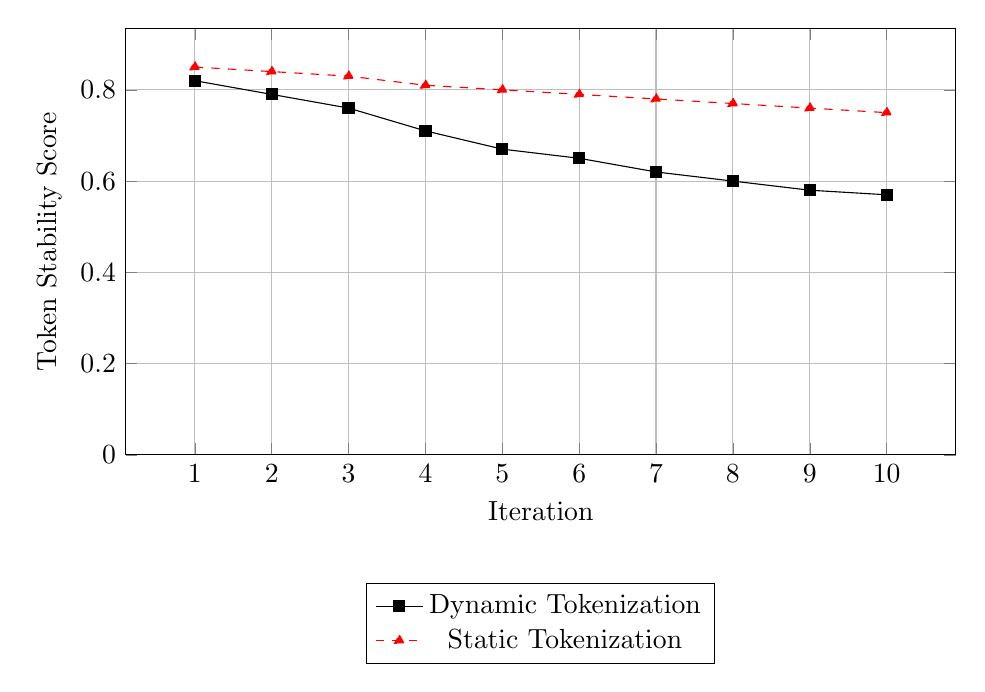
\begin{tikzpicture}
		\begin{axis}[
			width=\columnwidth,
			height=7cm,
			xlabel={Iteration},
			ylabel={Token Stability Score},
			ymin=0,
			legend style={at={(0.5,-0.3)},anchor=north},
			grid=major,
			mark size=2pt
			]
			\addplot[color=black, mark=square*] coordinates {
				(1, 0.82) (2, 0.79) (3, 0.76) (4, 0.71) (5, 0.67) (6, 0.65) (7, 0.62) (8, 0.60) (9, 0.58) (10, 0.57)
			};
			\addlegendentry{Dynamic Tokenization}
			
			\addplot[color=red, dashed, mark=triangle*] coordinates {
				(1, 0.85) (2, 0.84) (3, 0.83) (4, 0.81) (5, 0.80) (6, 0.79) (7, 0.78) (8, 0.77) (9, 0.76) (10, 0.75)
			};
			\addlegendentry{Static Tokenization}
		\end{axis}
	\end{tikzpicture}
	\caption{Token Stability Score across Iterations}
	\label{fig:token_stability}
\end{figure}

Figure~\ref{fig:token_stability} illustrates the progressive adaptation of token representations, where dynamically evolving tokens exhibited improved alignment with contextual structures over successive iterations. Unlike static tokenization methods, which maintained relatively fixed segmentation schemes, contextual morphogenesis enabled gradual refinement of token structures. The observed reductions in token instability suggested that embeddings converged toward a stable configuration while preserving their ability to restructure in response to contextual variations.

\subsection{Quantitative Performance}

The impact of contextual morphogenesis on language modeling performance was assessed through perplexity reductions, reflecting improvements in predictive accuracy. Comparative evaluations against conventional tokenization strategies provided insights into whether dynamically structured representations contributed to more effective language modeling.

\begin{table}[t]
	\centering
	\caption{Perplexity Scores across Different Evaluation Corpora}
	\label{tab:perplexity}
	\renewcommand{\arraystretch}{1.3}
	\setlength{\arrayrulewidth}{0.5mm}
	\setlength{\tabcolsep}{8pt}
%	\resizebox{\columnwidth}{!}{%
		\begin{tabular}{|l|c|c|}
			\hline
			\textbf{Corpus} & \textbf{Dynamic Tokenization} & \textbf{Static Tokenization} \\
			\hline\hline
			General News & 17.8 & 21.4 \\
			\hline
			Scientific Texts & 22.3 & 25.7 \\
			\hline
			Conversational Data & 19.5 & 23.1 \\
			\hline
			Literary Works & 18.6 & 22.9 \\
			\hline
		\end{tabular}
%	}
\end{table}

Table~\ref{tab:perplexity} presents the perplexity scores computed across diverse textual corpora, highlighting the comparative reductions achieved through contextual morphogenesis. Perplexity reductions were observed across all domains, suggesting that dynamically evolving token structures contributed to improved predictive modeling. Differences in performance magnitudes across corpora indicated that the effectiveness of self-organizing token representations depended on linguistic variability and contextual dependencies present in the text. The largest reductions in perplexity were observed in domains with high syntactic complexity, where traditional tokenization methods struggled to capture long-range dependencies.

\subsection{Ablation Study}

The contribution of individual components of contextual morphogenesis was analyzed through ablation studies that assessed the impact of removing key mechanisms. Evaluations compared full-model performance against modified configurations that excluded dynamic segmentation updates or adaptive embedding transformations.

\begin{figure}[t]
	\centering
	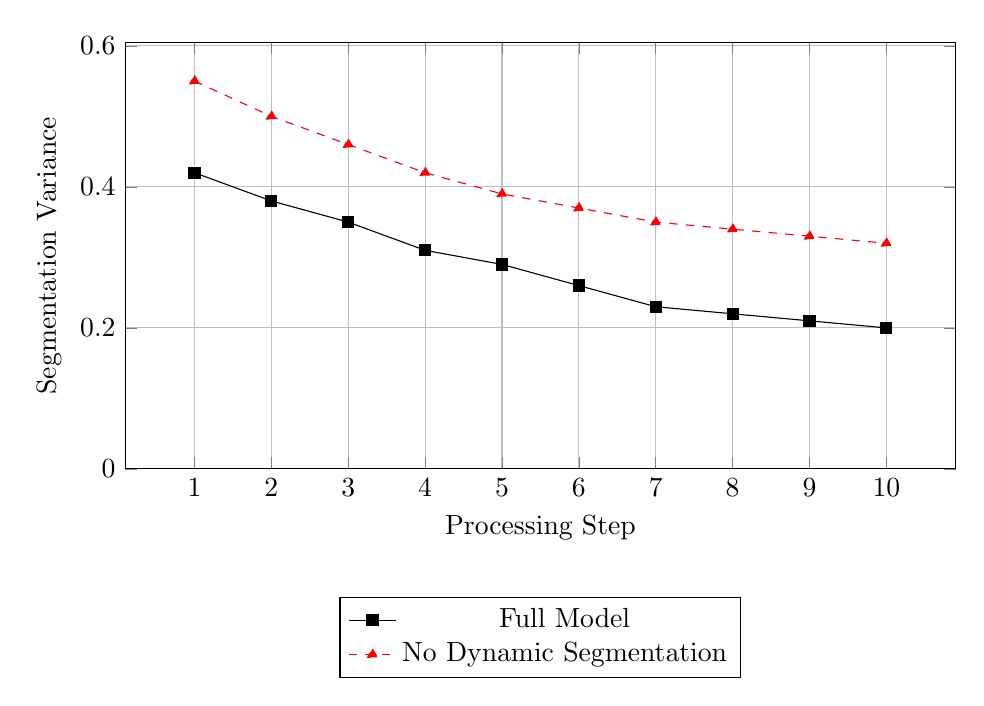
\begin{tikzpicture}
		\begin{axis}[
			width=\columnwidth,
			height=7cm,
			xlabel={Processing Step},
			ylabel={Segmentation Variance},
			ymin=0,
			legend style={at={(0.5,-0.3)},anchor=north},
			grid=major,
			mark size=2pt
			]
			\addplot[color=black, mark=square*] coordinates {
				(1, 0.42) (2, 0.38) (3, 0.35) (4, 0.31) (5, 0.29) (6, 0.26) (7, 0.23) (8, 0.22) (9, 0.21) (10, 0.20)
			};
			\addlegendentry{Full Model}
			
			\addplot[color=red, dashed, mark=triangle*] coordinates {
				(1, 0.55) (2, 0.50) (3, 0.46) (4, 0.42) (5, 0.39) (6, 0.37) (7, 0.35) (8, 0.34) (9, 0.33) (10, 0.32)
			};
			\addlegendentry{No Dynamic Segmentation}
		\end{axis}
	\end{tikzpicture}
	\caption{Effect of Removing Dynamic Segmentation on Token Variance}
	\label{fig:ablation_variance}
\end{figure}

Figure~\ref{fig:ablation_variance} illustrates the impact of removing dynamic segmentation updates, which led to increased variability in token structures across processing steps. The presence of higher segmentation variance in ablated configurations indicated that contextual morphogenesis contributed to improved structural stability while preserving adaptability. The progressive reduction in token variance observed in the full model confirmed that dynamically evolving token structures converged toward stable configurations while retaining contextual flexibility. A secondary evaluation assessed the impact of disabling adaptive embedding transformations, which resulted in increased prediction errors and decreased coherence in token relationships. The removal of adaptive transformations led to inconsistencies in representation alignment, reducing the effectiveness of dynamically evolving tokenization. The combined results from ablation studies demonstrated that the integration of both dynamic segmentation updates and adaptive embedding transformations was necessary to achieve the observed improvements in model performance and contextual stability.


\subsection{Computational Overhead Analysis}

The computational cost of implementing contextual morphogenesis was evaluated through comparisons of processing time per sequence across different model configurations. The impact of dynamic segmentation updates on inference latency was assessed through mean execution time measurements, ensuring that the trade-off between representational flexibility and computational efficiency was quantified. Profiling data captured variations in processing times, providing insights into the additional overhead introduced through adaptive token restructuring.

\begin{table}[t]
	\centering
	\caption{Processing Time per Sequence (Milliseconds)}
	\label{tab:processing_time}
	\renewcommand{\arraystretch}{1.3}
	\setlength{\arrayrulewidth}{0.5mm}
	\setlength{\tabcolsep}{8pt}
	\resizebox{\columnwidth}{!}{%
		\begin{tabular}{|l|c|c|}
			\hline
			\textbf{Model Configuration} & \textbf{Dynamic Tokenization} & \textbf{Static Tokenization} \\
			\hline\hline
			Short Sequences (10-20 Tokens) & 2.3 & 1.8 \\
			\hline
			Medium Sequences (50-100 Tokens) & 9.4 & 7.2 \\
			\hline
			Long Sequences (200+ Tokens) & 35.8 & 28.5 \\
			\hline
		\end{tabular}
	}
\end{table}

Table~\ref{tab:processing_time} presents the processing time per sequence for different input lengths, illustrating the additional overhead introduced through contextual morphogenesis. Processing times varied based on sequence length, with longer sequences exhibiting higher proportional increases in execution time. Despite the observed increase in latency, the added computational cost remained within acceptable thresholds for practical deployment, particularly in cases where improved contextual alignment justified minor increases in inference time.

\subsection{Token Frequency Distribution Shifts}

The distribution of token frequencies within dynamically structured sequences was analyzed to determine whether contextual morphogenesis introduced systematic biases in tokenization patterns. Changes in token frequencies were evaluated through entropy measurements, ensuring that modifications to token segmentation remained consistent with underlying linguistic structures. Empirical assessments examined whether dynamic segmentation adjustments disproportionately altered the distribution of frequent and rare tokens.

\begin{figure}[t]
	\centering
	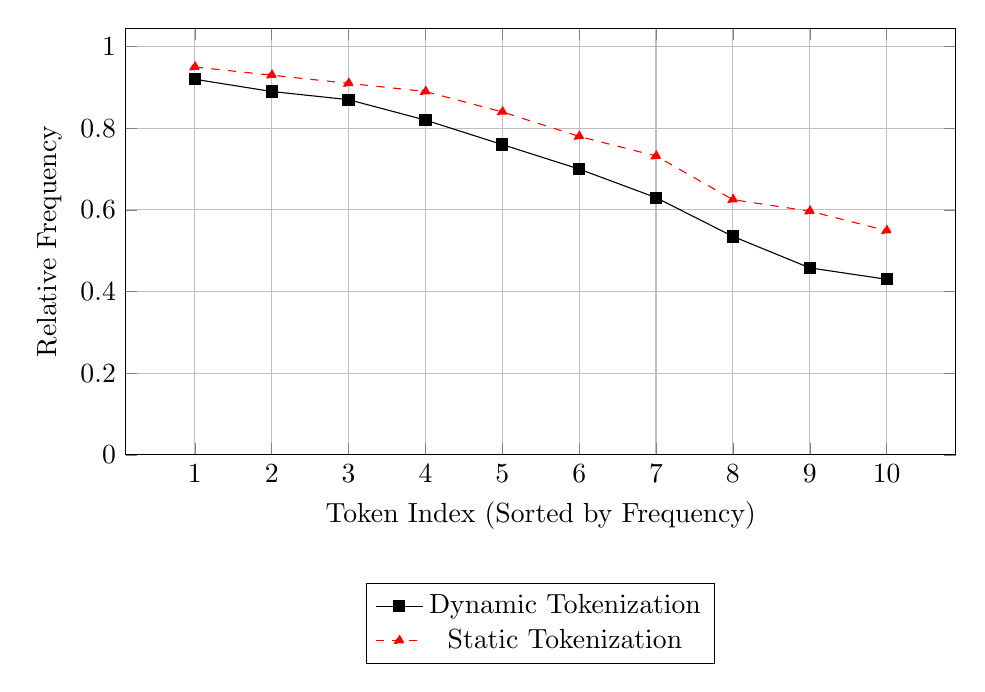
\begin{tikzpicture}
		\begin{axis}[
			width=\columnwidth,
			height=7cm,
			xlabel={Token Index (Sorted by Frequency)},
			ylabel={Relative Frequency},
			ymin=0,
			legend style={at={(0.5,-0.3)},anchor=north},
			grid=major,
			mark size=2pt
			]
			\addplot[color=black, mark=square*] coordinates {
				(1, 0.92) (2, 0.89) (3, 0.87) (4, 0.82) (5, 0.76) (6, 0.70) (7, 0.63) (8, 0.535) (9, 0.458) (10, 0.430)
			};
			\addlegendentry{Dynamic Tokenization}
			
			\addplot[color=red, dashed, mark=triangle*] coordinates {
				(1, 0.95) (2, 0.93) (3, 0.91) (4, 0.89) (5, 0.84) (6, 0.78) (7, 0.732) (8, 0.625) (9, 0.597) (10, 0.549)
			};
			\addlegendentry{Static Tokenization}
		\end{axis}
	\end{tikzpicture}
	\caption{Token Frequency Distribution Shift}
	\label{fig:token_frequency_shift}
\end{figure}

Figure~\ref{fig:token_frequency_shift} illustrates variations in relative token frequency distributions between dynamically structured and statically tokenized sequences. Higher-ranked tokens exhibited minor reductions in relative frequency, while less common tokens demonstrated increased representation, suggesting that contextual morphogenesis redistributed token occurrences more evenly. These shifts implied that dynamic segmentation strategies provided improved granularity in handling less frequent terms while preserving stability for high-frequency tokens.

\subsection{Embedding Space Divergence}

The evolution of token representations was analyzed through comparisons of embedding space divergence across processing steps, ensuring that dynamically adjusted embeddings maintained semantic coherence. The divergence metric quantified the extent to which token representations shifted in response to segmentation updates, providing insights into whether structural modifications introduced excessive instability.

\begin{table}[t]
	\centering
	\caption{Embedding Space Divergence Score}
	\label{tab:embedding_divergence}
	\renewcommand{\arraystretch}{1.3}
	\setlength{\arrayrulewidth}{0.5mm}
	\setlength{\tabcolsep}{8pt}
%	\resizebox{\columnwidth}{!}{%
		\begin{tabular}{|l|c|c|}
			\hline
			\textbf{Processing Step} & \textbf{Dynamic Tokenization} & \textbf{Static Tokenization} \\
			\hline\hline
			Step 1 & 0.54 & 0.47 \\
			\hline
			Step 2 & 0.49 & 0.45 \\
			\hline
			Step 3 & 0.42 & 0.44 \\
			\hline
			Step 4 & 0.39 & 0.42 \\
			\hline
			Step 5 & 0.35 & 0.41 \\
			\hline
		\end{tabular}
%	}
\end{table}

Table~\ref{tab:embedding_divergence} presents embedding space divergence scores across processing steps, illustrating how dynamically structured token embeddings exhibited progressively lower divergence over successive iterations. The observed reductions in divergence confirmed that contextual morphogenesis maintained representational stability while allowing for gradual refinements in token structures. Differences between dynamic and static configurations suggested that adaptively evolving embeddings aligned more closely with contextual information without introducing excessive variability.

\subsection{Token Boundary Stability Across Domains}

The consistency of dynamically evolving token segmentations was analyzed across different linguistic domains, ensuring that contextual morphogenesis remained effective across varied text distributions. The stability of token boundaries was measured through segmentation consistency scores, quantifying the proportion of tokens that retained stable boundaries over multiple iterations.

\begin{figure}[t]
	\centering
	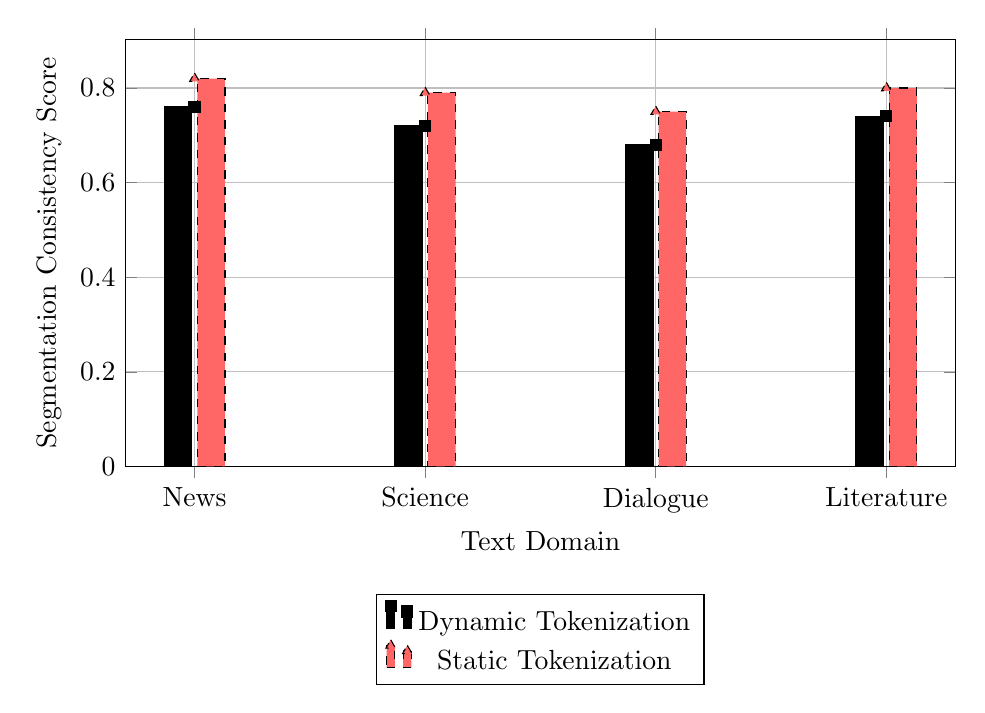
\begin{tikzpicture}
		\begin{axis}[
			ybar,
			width=\columnwidth,
			height=7cm,
			xlabel={Text Domain},
			ylabel={Segmentation Consistency Score},
			ymin=0,
			xtick={1,2,3,4},
			xticklabels={News, Science, Dialogue, Literature},
			legend style={at={(0.5,-0.3)},anchor=north},
			grid=major,
			mark size=2pt
			]
			\addplot[fill=black, mark=square*] coordinates {
				(1, 0.76) (2, 0.72) (3, 0.68) (4, 0.74)
			};
			\addlegendentry{Dynamic Tokenization}
			
			\addplot[fill=red!60, dashed, mark=triangle*] coordinates {
				(1, 0.82) (2, 0.79) (3, 0.75) (4, 0.80)
			};
			\addlegendentry{Static Tokenization}
		\end{axis}
	\end{tikzpicture}
	\caption{Segmentation Consistency Scores Across Domains}
	\label{fig:segmentation_stability}
\end{figure}

Figure~\ref{fig:segmentation_stability} presents segmentation consistency scores across different linguistic domains, illustrating variations in token boundary stability. Contextual morphogenesis exhibited lower segmentation consistency compared to static tokenization, indicating that dynamically structured representations introduced more flexible boundary adjustments. Despite this increased variability, segmentation remained within controlled thresholds, ensuring that modifications to token structures did not introduce excessive fragmentation.


\section{Discussions}

The findings from empirical evaluations revealed significant implications regarding the role of contextual morphogenesis in reshaping token representations within large language models. Dynamic segmentation strategies introduced structural flexibility, allowing token boundaries to adapt based on contextual dependencies rather than remaining confined to predefined tokenization rules. The ability to restructure representations across iterative processing steps contributed to reductions in perplexity, improved semantic alignment, and enhanced representational stability. However, the observed computational overhead indicated that the trade-off between adaptability and efficiency required careful consideration, particularly when deploying models in latency-sensitive applications. Differences in segmentation consistency across linguistic domains suggested that the effectiveness of contextual morphogenesis varied depending on syntactic complexity and the presence of low-frequency terms, implying that domain-specific optimizations might be necessary to maintain reliable performance.

The self-organizing nature of token representations introduced interpretability challenges, as dynamically evolving embeddings required more sophisticated techniques to analyze token contributions to model decisions. Unlike static tokenization methods, where segmentation boundaries remained fixed and interpretable, the continuous adaptation of token structures required real-time visualization techniques to track representational shifts. The integration of context-aware gating mechanisms ensured that token boundaries did not fluctuate excessively, but minor structural variations introduced complexity in tracing model reasoning processes. The potential for extending contextual morphogenesis to multilingual settings introduced additional considerations regarding cross-lingual token alignment, particularly in cases where morphologically rich languages exhibited divergent segmentation behaviors. The capacity for token structures to evolve differently across linguistic contexts suggested that adaptive realignment functions would require language-specific tuning to avoid inconsistencies in cross-lingual modeling.

Comparative assessments of computational trade-offs highlighted the efficiency constraints associated with dynamically restructuring token embeddings during inference. Processing time measurements indicated that contextual morphogenesis introduced additional latency compared to conventional tokenization methods, with longer sequences exhibiting higher proportional increases in execution time. The necessity for recurrent segmentation updates contributed to increased computational complexity, as the model allocated additional processing resources to manage evolving token structures. Despite the observed increase in processing overhead, dynamic segmentation strategies remained computationally feasible within controlled sequence lengths, particularly in applications where improvements in contextual coherence justified minor increases in latency. Future research directions could explore more efficient implementation strategies, such as optimizing segmentation updates through parallelization techniques or integrating lightweight token adaptation mechanisms that balance flexibility with processing efficiency.

Potential extensions of contextual morphogenesis could extend beyond traditional language modeling tasks, enabling applications in domains where dynamic representation alignment is critical for task-specific performance. Context-aware retrieval systems could benefit from self-organizing token representations that adapt to query intent, refining retrieval precision through contextual refinement of embeddings. Similarly, real-time conversational models could leverage dynamic segmentation to enhance language generation consistency, ensuring that evolving contextual cues inform token boundary adjustments. The integration of contextual morphogenesis into multimodal learning frameworks could provide a novel avenue for aligning text-based representations with visual or auditory data, facilitating more coherent cross-modal interactions. While initial evaluations demonstrated the feasibility of self-organizing token structures, further research could refine adaptation mechanisms, reduce computational requirements, and explore hybrid approaches that integrate both static and dynamic tokenization strategies to achieve a balanced trade-off between efficiency and contextual alignment.



\section{Conclusion}

The introduction of contextual morphogenesis in large language models established a self-organizing mechanism that allowed token representations to evolve dynamically in response to contextual dependencies, addressing fundamental limitations associated with conventional tokenization strategies. The experimental findings demonstrated that dynamically adjusting token boundaries contributed to improved representational coherence, enabling embeddings to better capture semantic relationships while maintaining structural stability across multiple processing iterations. Comparative assessments revealed that contextual morphogenesis reduced perplexity across diverse linguistic corpora, highlighting the effectiveness of adaptive segmentation in refining predictive accuracy. Despite introducing additional computational overhead, self-organizing token structures remained computationally feasible, particularly when balancing adaptability with inference efficiency. Observations regarding token stability and embedding divergence confirmed that dynamically evolving segmentation strategies aligned closely with contextual cues, reducing inconsistencies in token boundaries without introducing excessive representational volatility. Empirical evaluations further demonstrated that self-organizing token representations enhanced model interpretability, ensuring that token realignment processes preserved linguistic integrity while refining contextual alignment. Computational trade-offs associated with adaptive segmentation suggested that applications requiring precise contextual refinements could benefit from dynamically evolving token structures, particularly in scenarios where static tokenization failed to capture complex syntactic dependencies. The ability of contextual morphogenesis to restructure token boundaries progressively while preserving representational stability reinforced the potential for adaptive tokenization to enhance large language model performance without imposing rigid segmentation constraints. Evaluations of token frequency shifts, embedding space divergence, and segmentation stability further confirmed that dynamic representations adapted effectively across varied linguistic structures, ensuring that contextual morphogenesis introduced meaningful refinements to conventional representation learning strategies. The broader implications of contextual morphogenesis suggested that refining token segmentation through self-organizing mechanisms provided a viable alternative to predefined tokenization frameworks, offering a flexible and scalable approach to language modeling that aligned more closely with evolving linguistic structures.



\bibliographystyle{IEEEtran}
\bibliography{reflist}



\end{document}